\section{Introdução}

\subsection{Motivação}

\begin{frame}

  \begin{itemize}
  \item Se uma imagem vale mais que 1000 palavras, então um recurso
    interativo vale mais que 1000 imagens
  \item Oferecer recursos para pessoas com menor proeficiência de
    programação
  \item Recursos web não requerem instalação/conhecimento em R
  \end{itemize}

\end{frame}

\subsection{Conteúdo}

\begin{frame}
\vspace{-1.0cm}

\begin{columns}[t]
\begin{column}{.3\textwidth}
\\ \vspace{1cm}
	Recursos interativos
  
  \begin{itemize}
  \setbeamercovered{transparent=35}
    \uncover<2>{
      \item \texttt{animation}
      }
    \uncover<3>{
      \item \texttt{rgl}
      }
    \uncover<4>{
      \item \texttt{googleVis}
      }
    \uncover<5>{
      \item \texttt{gWidgets}
      }
    \uncover<6>{
      \item \texttt{rpanel}
      }
    \uncover<7>{
      \item \texttt{shiny}
      }
     \end{itemize}
     \vspace{1cm}
\end{column}

\begin{column}{.6\textwidth}
\\ \vspace{0.5cm}
    \only<2>{
      {\center
      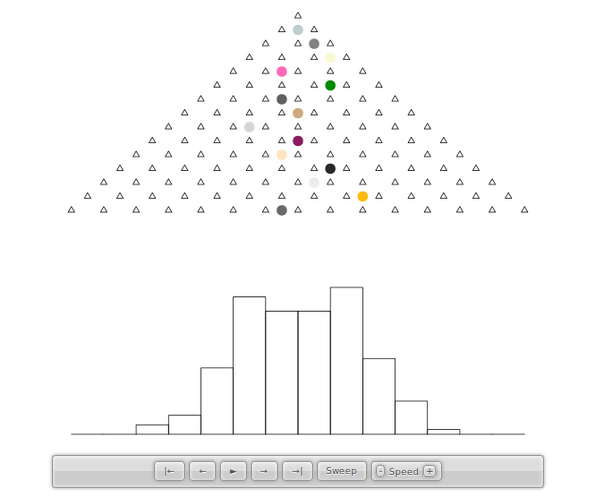
\includegraphics[scale=0.3]{images/preview_ani}}}
    \only<3>{
      {\center
      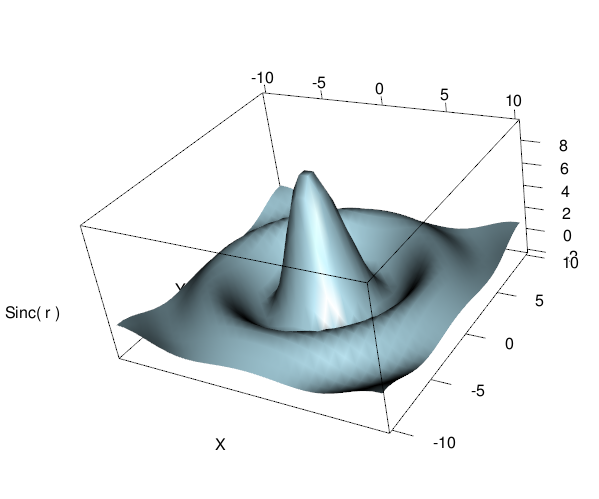
\includegraphics[scale=0.3]{images/preview_rgl}}}
    \only<4>{
      {\center 
      \vspace{-0.7cm}
      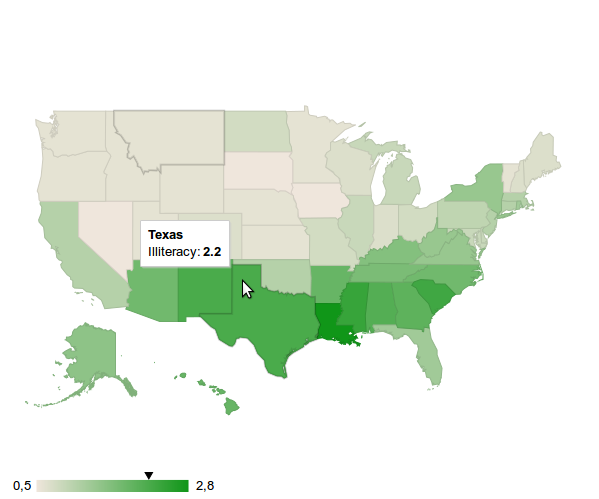
\includegraphics[scale=0.3]{images/preview_ggvis}}}
    \only<5>{
      {\center
      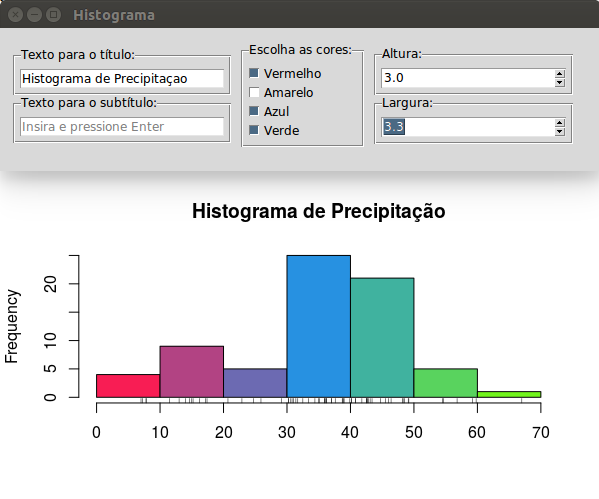
\includegraphics[scale=0.3]{images/preview_gwidgets}}}
    \only<6>{
      {\center
      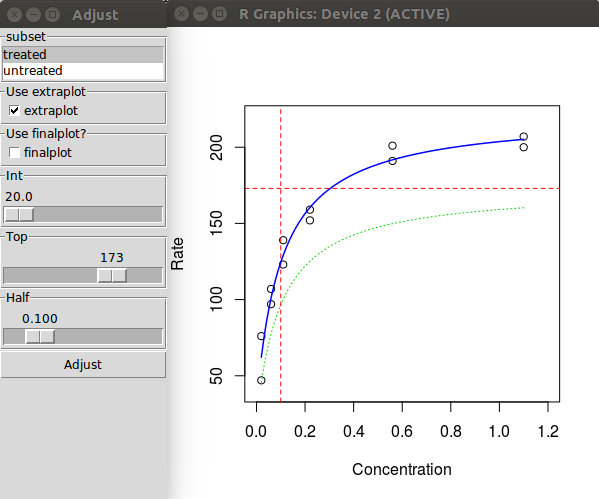
\includegraphics[scale=0.3]{images/preview_rpanel}}}
    \only<7>{
      {\center
      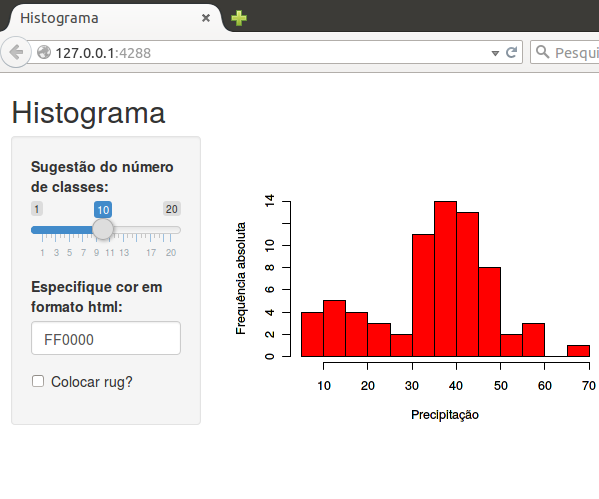
\includegraphics[scale=0.3]{images/preview_shiny}}}
\end{column}
    \end{columns}

\end{frame}

\subsection{Recursos interativos básicos}

\begin{frame}

  \begin{itemize}
  \item \texttt{locator()} e \texttt{identify()}
  \item \texttt{readline()}
  \item \texttt{for} e \texttt{while} com \texttt{Sys.sleep()}
  \end{itemize}

\end{frame}
